\documentclass{beamer}
\setbeamertemplate{navigation symbols}{}
%\usetheme{m}

\usepackage{beamerthemeshadow}
\usepackage{nth}
\usepackage[export]{adjustbox}

\def\beamer@andinst{\quad}
\makeatother

\newcommand\parallelcontent[2]{
  \begin{columns}[t]
    \column{0.48\textwidth} #1
    \column{0.48\textwidth} #2
  \end{columns}
}
\newcommand\parallelitem[2]{
  \parallelcontent
  {\begin{itemize} \item #1 \end{itemize}}
  {\begin{itemize} \item[] #2 \end{itemize}}
}

\begin{document}
\title{Diabetic Retinopathy Detection}
\subtitle{}  
\author[]{Sergey Ovcharenko \inst{1} \and Rasim Akhunzyanov \inst{2}}
\institute[shortinst]{\inst{1} Deep Learning Engineer at NTech Lab \and \inst{2} Computer Vision Research Engineer at LG Electronics}

\date{\today} 

\begin{frame}
\titlepage
\end{frame}

\begin{frame}
\frametitle{Table of contents}\tableofcontents
\end{frame} 


\section{Overview} 

\subsection{Competition Details}
\begin{frame}\frametitle{Data} 
\par Goal: Identify signs of diabetic retinopathy in eye images \\~\\
\par 35126 images = 17563 pairs for training
\par 53576 images in test set
\par 3 channel images
\par Images are big: 2500x2000
\par Evaluation: quadratic weighted kappa
\end{frame}

\subsection{Competition Results}
\begin{frame}\frametitle{} 
\par final leaderboard
\par + provide leaderboard histogram
\par + plot score over time
\end{frame}


\section{Approach} 
\subsection{Data preprocessing}
\begin{frame}\frametitle{Preprocessing}

\begin{enumerate}
\item Crop black borders
\item Resize
\item Optionally: crop internal square
\item Optionally: Local Contrast Normalization (LCN) $ \hat{I}_{x,y} = \frac{I_{x,y} - \mu_{x,y}}{\sigma_{x,y}} $
\end{enumerate}

\end{frame}

\begin{frame}{Preprocessing}

  \parallelcontent
  {} %\textcolor{red}{\rule{\linewidth}{4pt} foo}}
  {} %\textcolor{blue}{\rule{\linewidth}{4pt} bar}}
  \parallelitem
  {Crop black borders}
  { \begin{figure}[!ht]
    \centering
	\adjustbox{valign=m}{  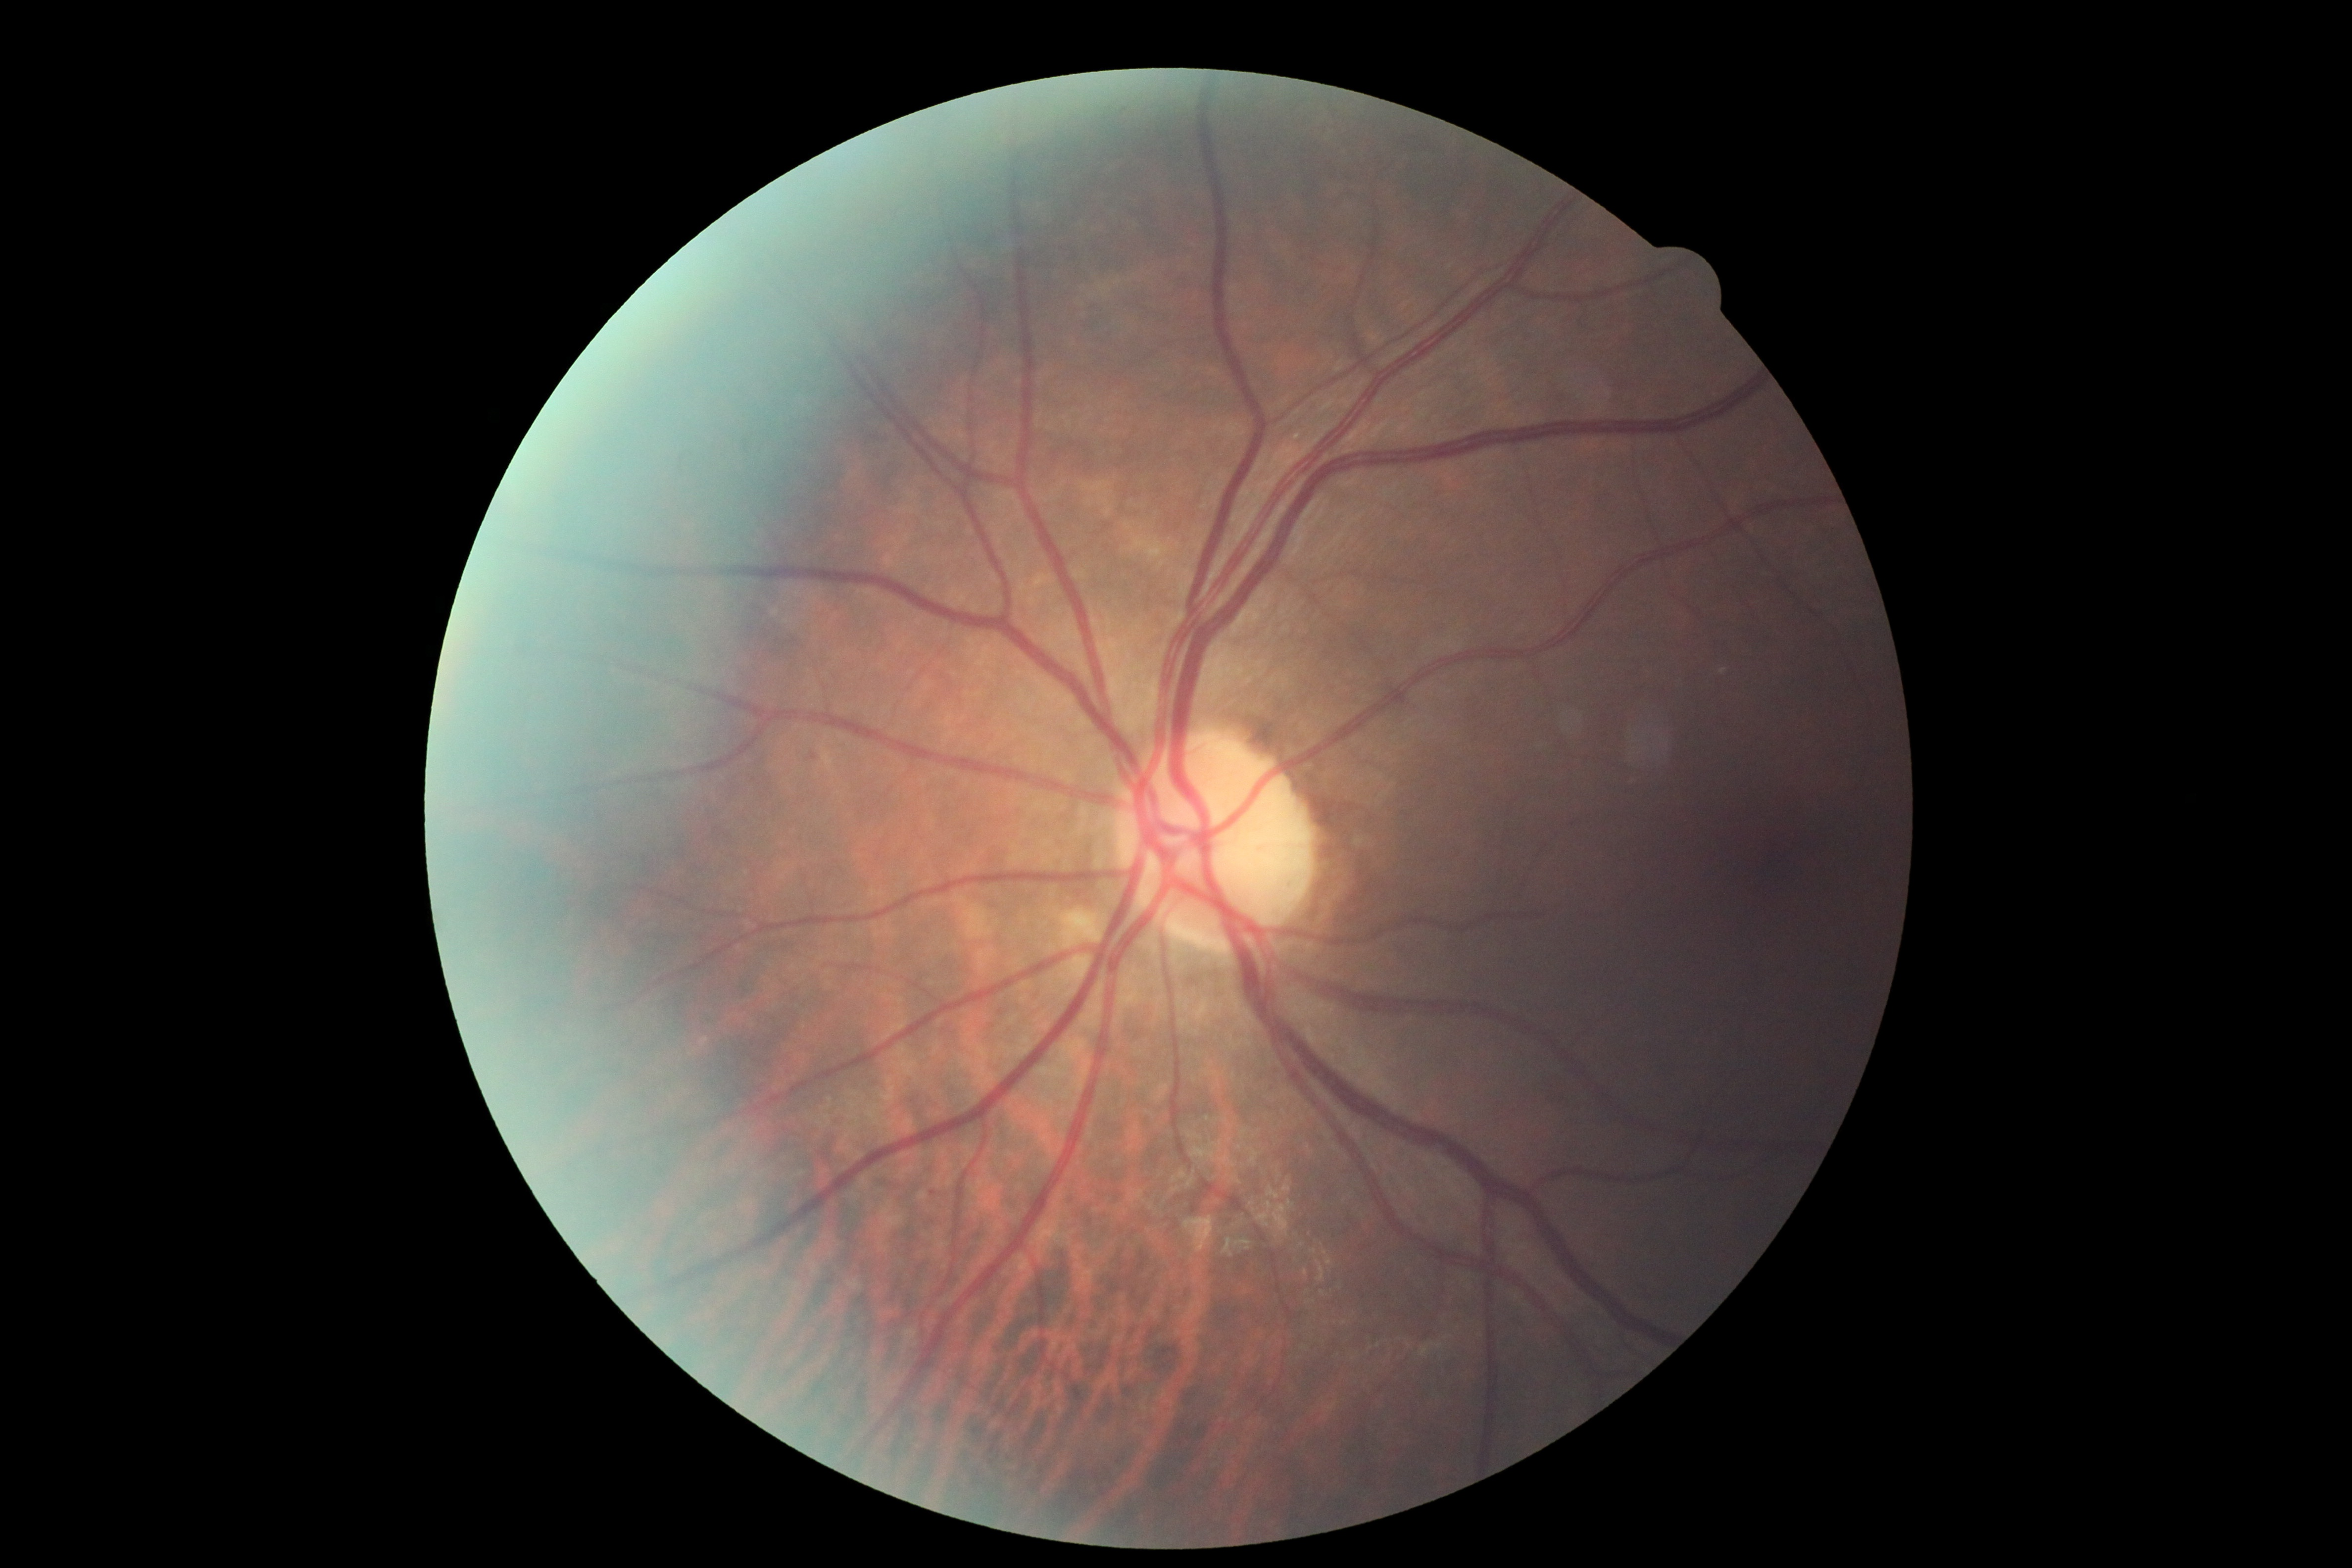
\includegraphics[valign=c,height=0.5cm]{pics/10_left.jpeg} }
    \adjustbox{valign=m}{ $\rightarrow$ }
    \adjustbox{valign=m}{ 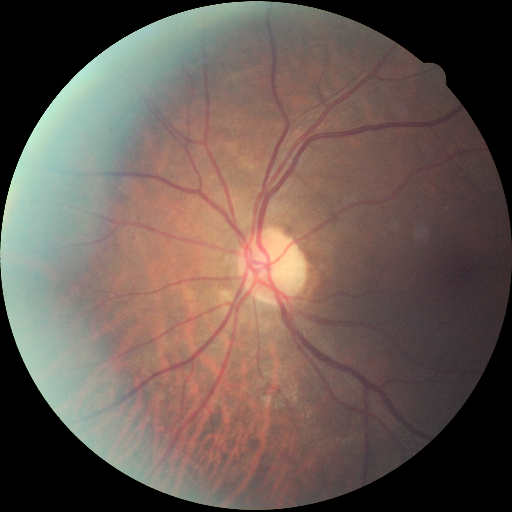
\includegraphics[valign=c,height=0.5cm]{pics/10_left.png} }
  \end{figure} }
  \parallelitem
  {Resize}
  {\begin{figure}[!ht]
      \centering
  	\adjustbox{valign=m}{  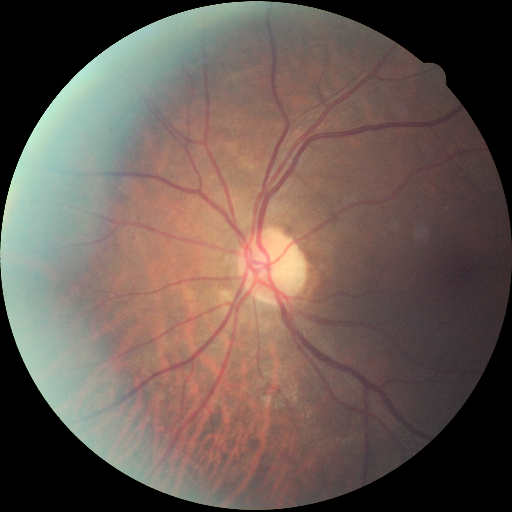
\includegraphics[valign=c,height=0.5cm]{pics/10_left.png} }
      \adjustbox{valign=m}{ $\rightarrow$ }
      \adjustbox{valign=m}{ 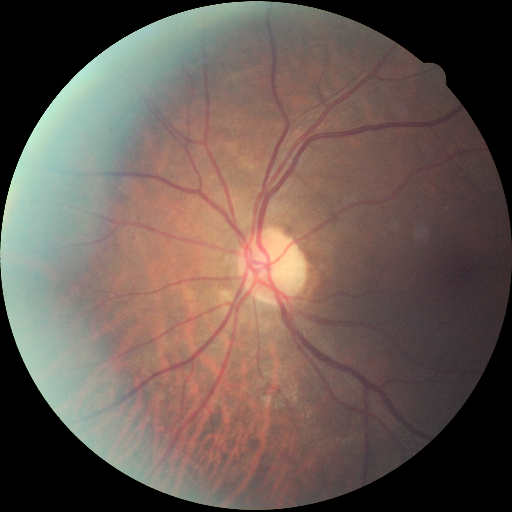
\includegraphics[valign=c,height=0.25cm]{pics/10_left.png} }
    \end{figure}}
  \parallelitem
  {Optionally: crop inscribed square}
  {\begin{figure}[!ht]
        \centering
    	\adjustbox{valign=m}{  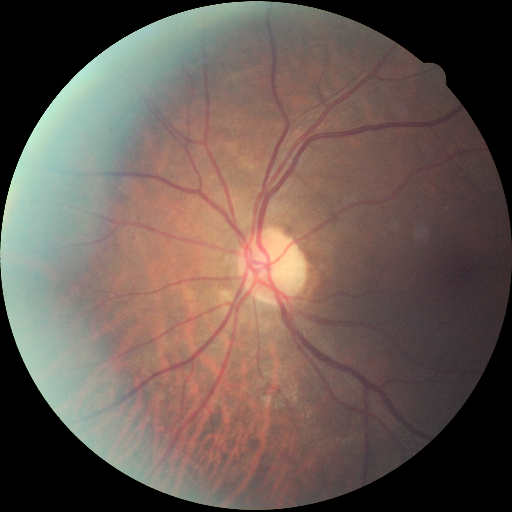
\includegraphics[valign=c,height=0.5cm]{pics/10_left.png} }
        \adjustbox{valign=m}{ $\rightarrow$ }
        \adjustbox{valign=m}{ 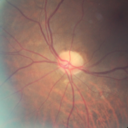
\includegraphics[valign=c,height=0.5cm]{pics/10_left_inner.png} }
      \end{figure}}
  \parallelitem
  {Optionally: Local Contrast Normalization (LCN) }
%  $ \hat{I}_{x,y} = \frac{I_{x,y} - \mu_{x,y}}{\sigma_{x,y}} $}
  { \begin{figure}[!ht]
      \centering
  	\adjustbox{valign=m}{  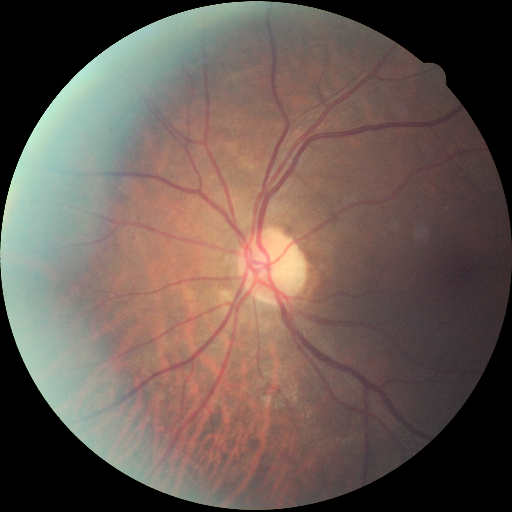
\includegraphics[valign=c,height=0.5cm]{pics/10_left.png} }
      \adjustbox{valign=m}{ $\rightarrow$ }
      \adjustbox{valign=m}{ 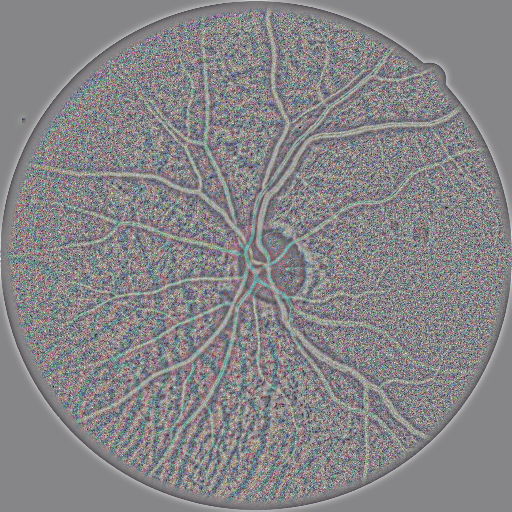
\includegraphics[valign=c,height=0.5cm]{pics/10_left_lcn.png} }
    \end{figure}
  }

\end{frame}

\begin{frame}\frametitle{Augmentation}
\begin{itemize}
\item Random mirror
\item Random rotation
\item Color augmentation - not helped
\end{itemize}

\end{frame}

\subsection{Network configuration}
\begin{frame}\frametitle{}
\par Slice rotate
\par Merge
\par Output
\end{frame}

\subsection{Decision making}

\begin{frame}\frametitle{}
\par Predict score for eyes independently
\par Final score = max(left, right)
\end{frame}

\section{Winning approaches} 
\subsection{\nth{1} place}
\subsection{\nth{2} place}
\subsection{\nth{3} place}

\section{Conclusions}

%
%
% Back up
% There are examples below to use in slides
%

\section{Back Up}

\begin{frame}\frametitle{Tables}
\begin{tabular}{|c|c|c|}
\hline
\textbf{Date} & \textbf{Instructor} & \textbf{Title} \\
\hline
WS 04/05 & Sascha Frank & First steps with  \LaTeX  \\
\hline
SS 05 & Sascha Frank & \LaTeX \ Course serial \\
\hline
\end{tabular}
\end{frame}

%\subsection{blocs}
\begin{frame}\frametitle{blocs}

\begin{block}{title of the bloc1}
bloc text
\end{block}

\begin{exampleblock}{title of the bloc2}
bloc text
\end{exampleblock}


\begin{alertblock}{title of the bloc3}
bloc text
\end{alertblock}

\end{frame}

%\subsection{split screen}

\begin{frame}\frametitle{splitting screen}
\begin{columns}
\begin{column}{5cm}
\begin{itemize}
\item Beamer 
\item Beamer Class 
\item Beamer Class Latex 
\end{itemize}
\end{column}
\begin{column}{5cm}
\begin{tabular}{|c|c|}
\hline
\textbf{Instructor} & \textbf{Title} \\
\hline
Sascha Frank &  \LaTeX \ Course 1 \\
\hline
Sascha Frank &  Course serial  \\
\hline
\end{tabular}
\end{column}
\end{columns}
\end{frame}

%\subsection{Pictures} 
\begin{frame}\frametitle{pictures in latex beamer class}
\begin{figure}
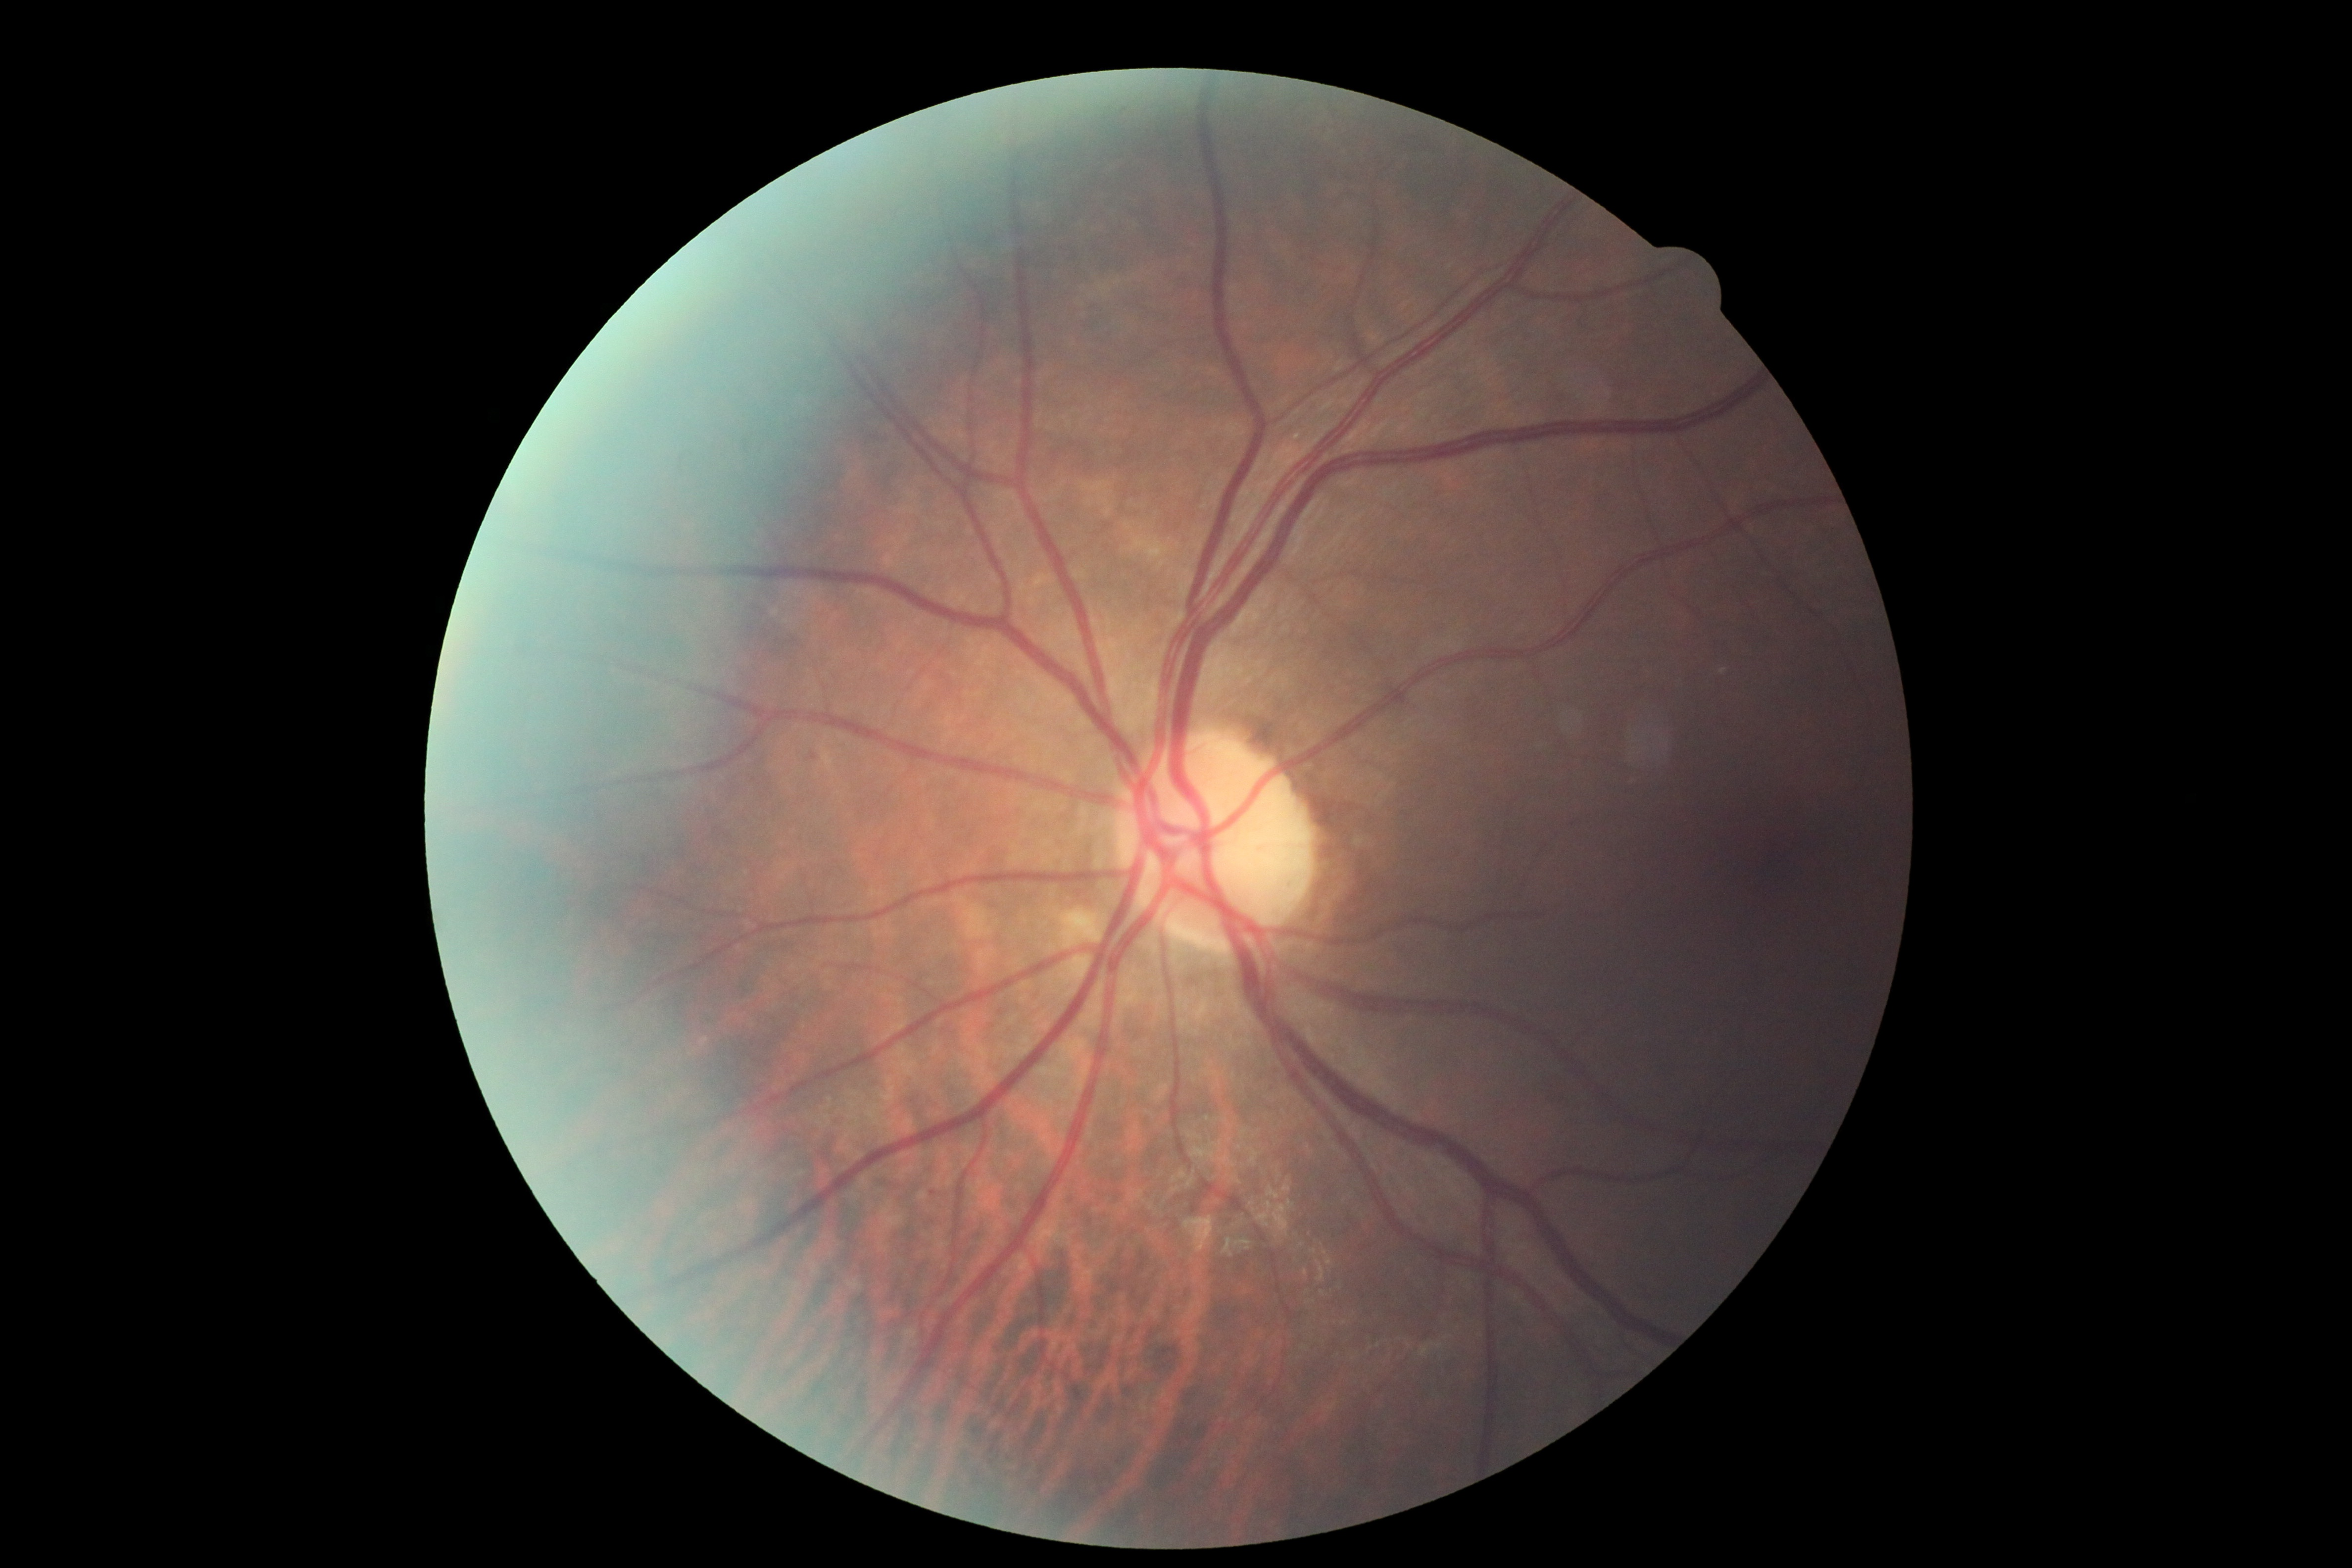
\includegraphics[scale=0.5]{pics/10_left.jpeg} 
\caption{show an example picture}
\end{figure}
\end{frame}

%\subsection{joining picture and lists} 

\begin{frame}
\frametitle{pictures and lists in beamer class}
\begin{columns}
\begin{column}{5cm}
\begin{itemize}
\item<1-> subject 1
\item<3-> subject 2
\item<5-> subject 3
\end{itemize}
\vspace{3cm} 
\end{column}
\begin{column}{5cm}
\begin{overprint}
\includegraphics<2>[width=2.5cm]{pics/10_left.jpeg}
\includegraphics<4>[width=2.5cm]{pics/10_left.jpeg}
\includegraphics<6>[width=2.5cm]{pics/10_left.jpeg}
\end{overprint}
\end{column}
\end{columns}
\end{frame}


%\subsection{pictures which need more space} 
\begin{frame}[plain]
\frametitle{plain, or a way to get more space}
\begin{figure}
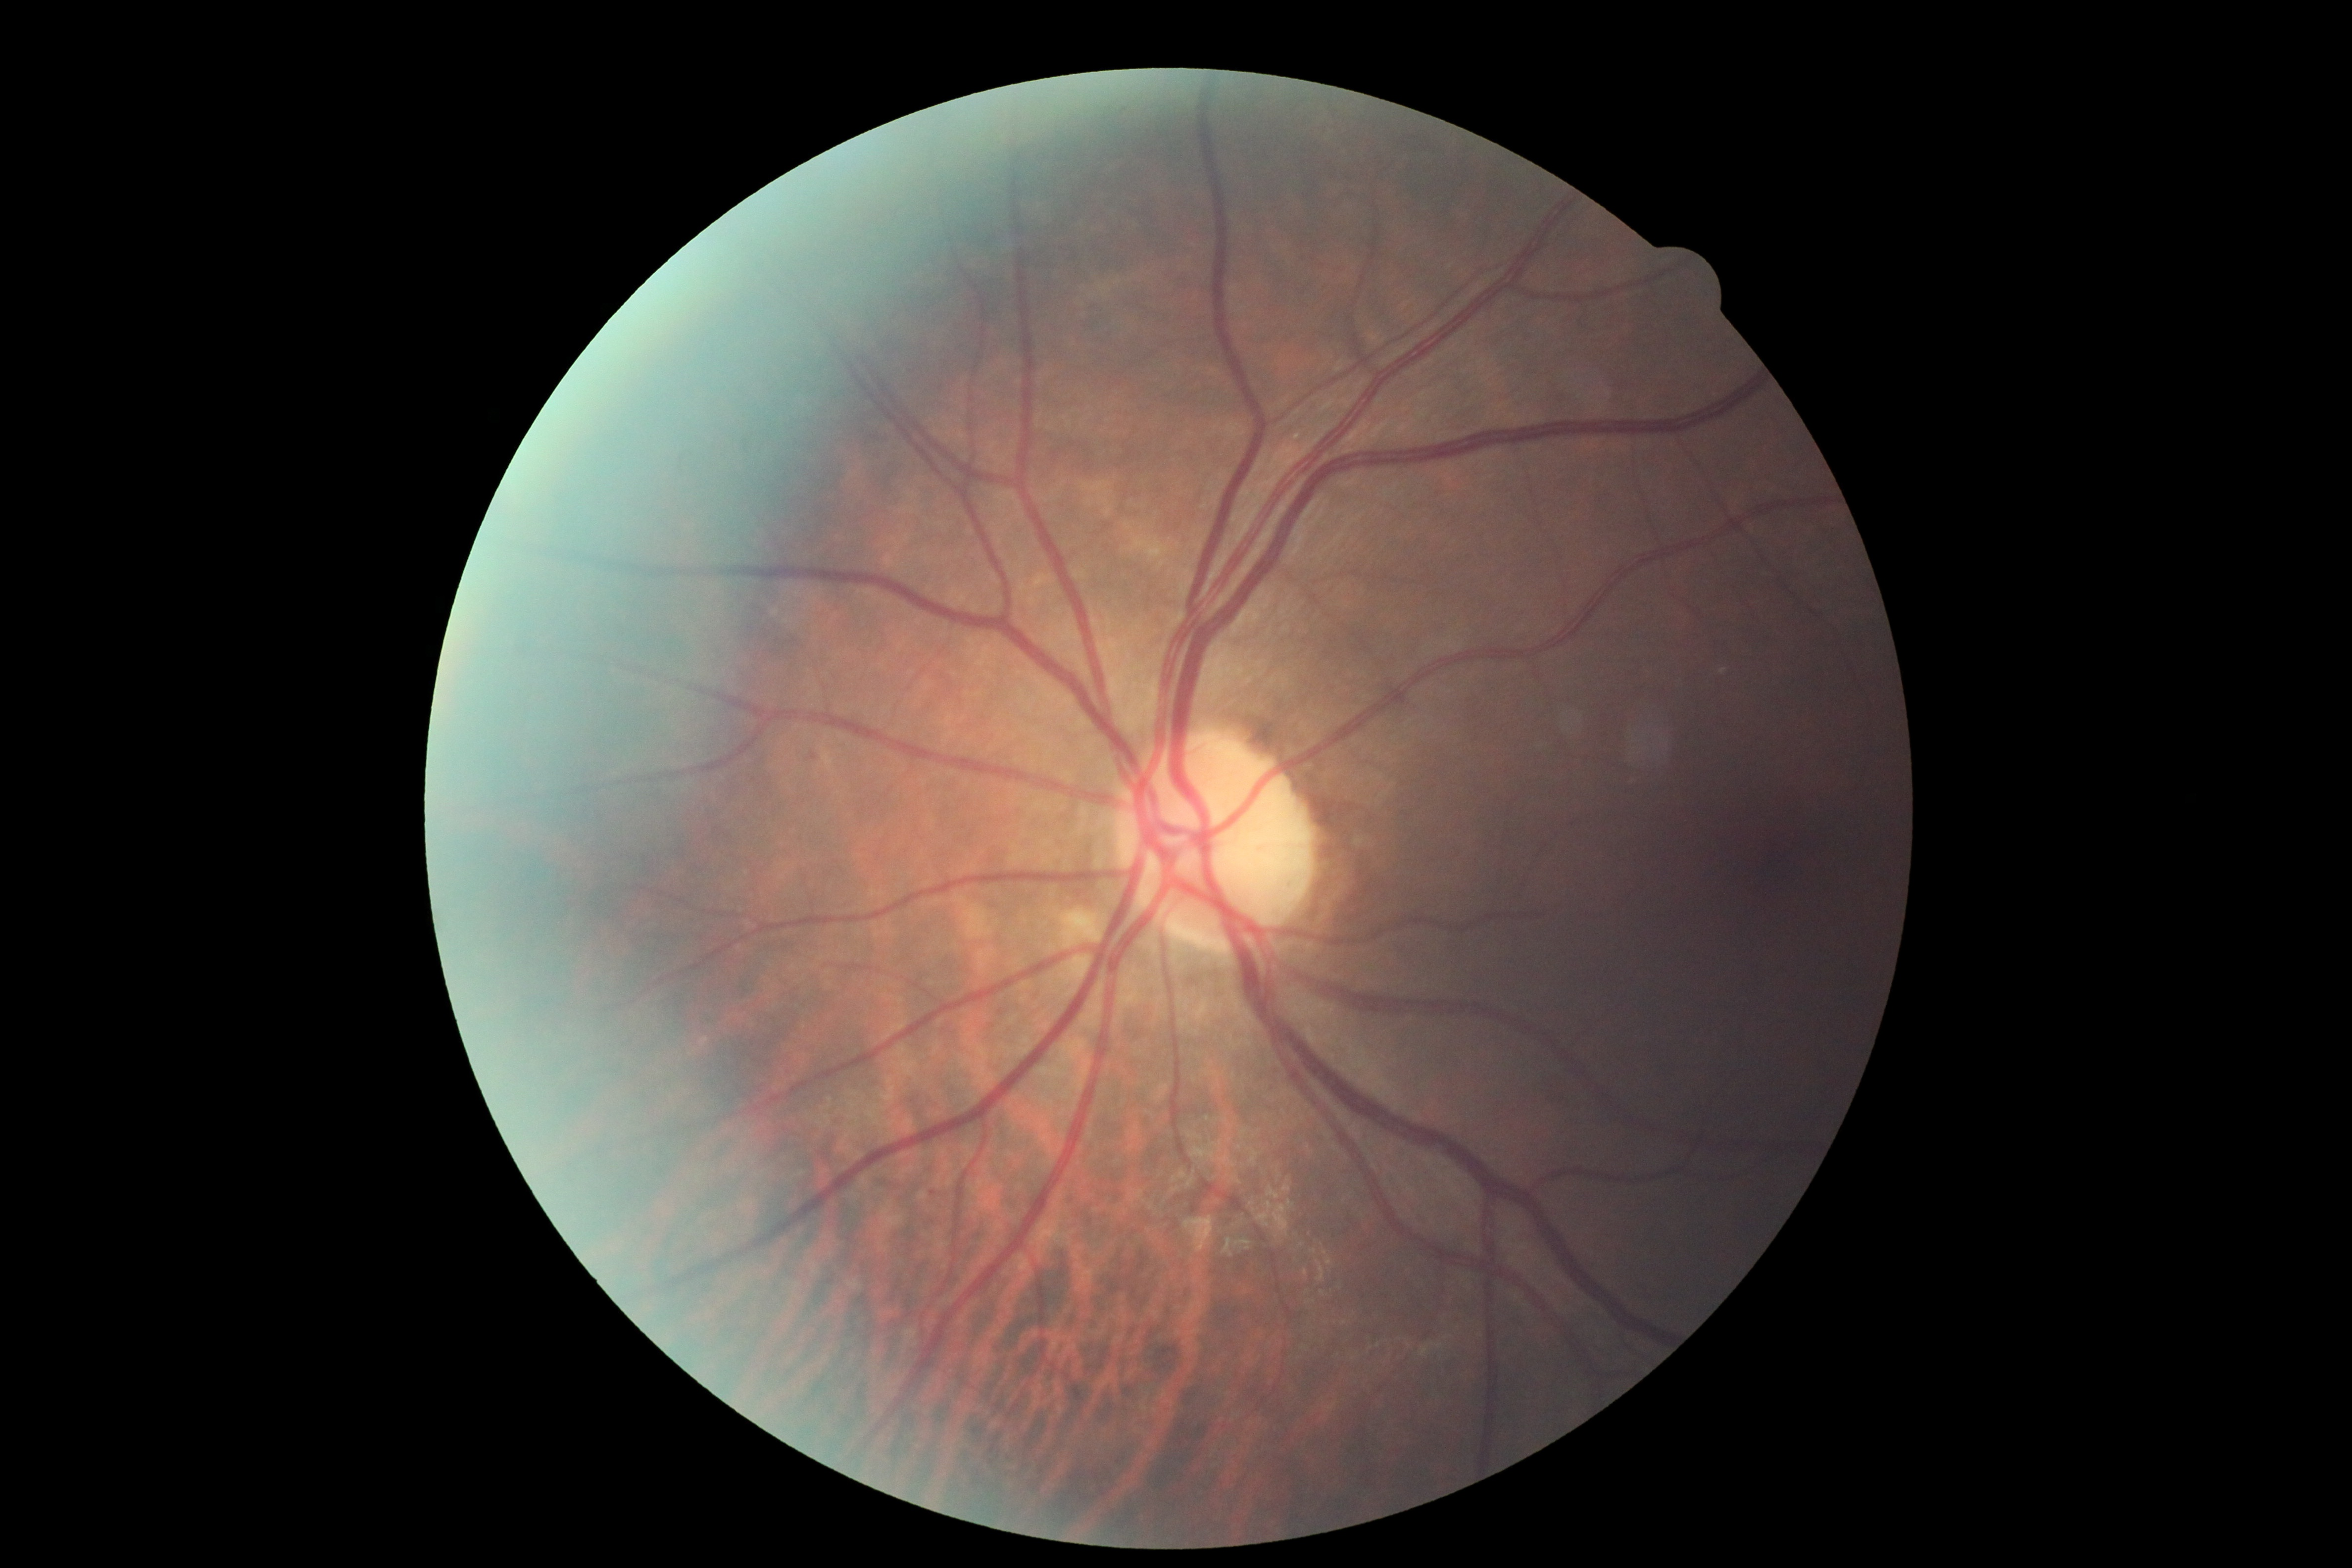
\includegraphics[scale=0.25]{pics/10_left.jpeg} 
\caption{show an example picture}
\end{figure}
\end{frame}



\end{document}